%%%%%%%%%%%%%%%%%%%%%%%%%%%%%%%%%%%%%%%%%%%%%%%%%%%%%%%%%%%%%%%%%%%%%%%%%%%%%%%%
% Implementation and algorithm details
%
%%%%%%%%%%%%%%%%%%%%%%%%%%%%%%%%%%%%%%%%%%%%%%%%%%%%%%%%%%%%%%%%%%%%%%%%%%%%%%%%


\chapter{Implementation}
In this section we discuss our implementation. We will briefly discuss our
system design architecture, followed by our modifications to the normal graphics
pipeline. Lastly we will discuss interesting problems that we encountered
and how we attempted to solve these problems. Finally we will discuss performance 
implications.

%%%%%%%%%%%%%%%%%%%%%%%%%%%%%%%%%%%%%%%%%%%%%%%%%%%%%%%%%%%%%%%%%%%%%%%%%%%%%%%
\section{Environment and Architecture}
The implementation of this prototype is done in the Java programming language.
Graphics are rendered through Java for OpenGL (JOGL) graphics library. A MySQL
database is used to host the text documents as well as their respective document
scores. Our graphics hardware is a NVIDIA Quadro FX video card. The prototype is
designed to run on 1680x1050 screen resolution. 

Our prototype implementation is a standard two-tier system: A persistence layer
and a user interface layer. The persistence layer is in charge of database
transactions, cached resources and system state. The user interface layer takes
care of the rendering tasks. 

    % === Figure === 
	\begin{figure}
	 \centering  
	 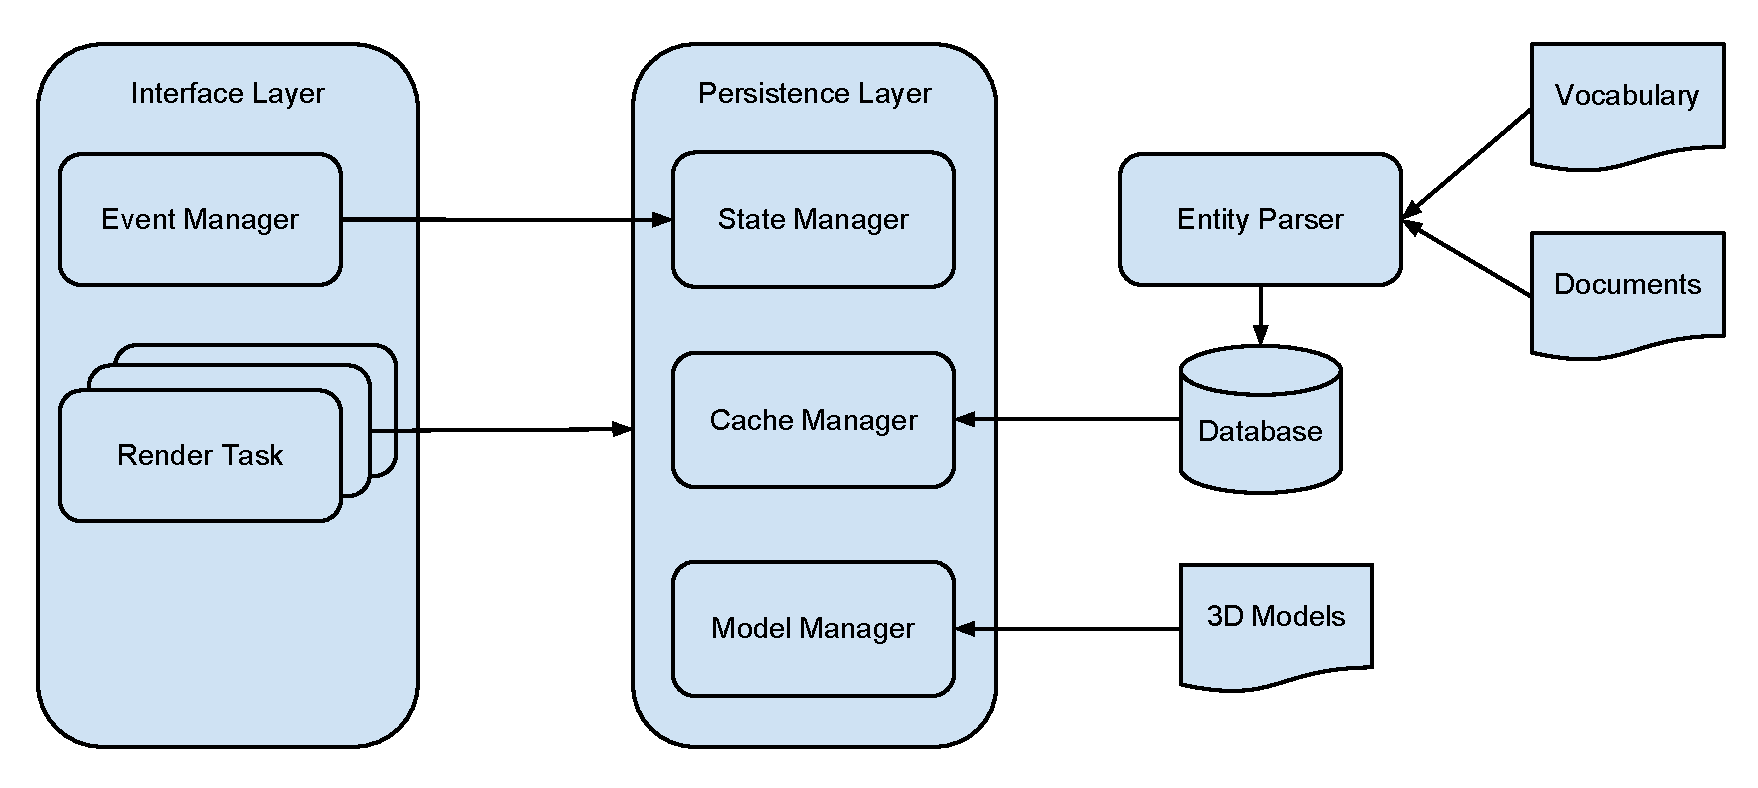
\includegraphics[width=2.5in]{Architecture.pdf} 
	 \caption{High level system architecture}
	 \label{figure:arch}
	\end{figure}
	% ==============

The major components of our system, as well as their functionalities are listed
below: 
\begin{itemize}[noitemsep]
  \item Render Task: Each rendering task is responsible for rendering a
  functional part of the user interface. Each task communicates with the
  persistence layer to retrieve updated states.
  \item State Manager: It keeps track of all data used for rendering and query
  building.
  \item Model Manager: Holds and manipulate model geometries.
  \item Cache Manager: Stores cache and handles database transactions.
  \item Event Manager: Listens for events, it dispatches changes to the State
  Manager.
\end{itemize}




%%%%%%%%%%%%%%%%%%%%%%%%%%%%%%%%%%%%%%%%%%%%%%%%%%%%%%%%%%%%%%%%%%%%%%%%%%%%%%%
\section{Algorithms}
During the development of the software prototype, we have encountered several
non-trivial problems. While these issues are not a part of our visualization 
design, they nonetheless impact the overall user experience via the degradation 
of aesthetic and usability of the application. In this section we discuss these 
problems and our proposed solutions.

\subsection{Order Independent Transparency}
We have mentioned briefly that rendering translucent geometries in 3D space can
create artifacts, here we will describe this in greater detail and outline 
possible solutions.
First of all, to create a translucent effect, we need to do two things: 
\begin{itemize} [noitemsep]
  \item Enable Blending: This option allows foreground object to blend with
  background objects.
  \item Disable Depth Testing: This option renders all geometries regardless of
  depth and overlaps.
\end{itemize}
Geometries are typically not sent to the hardware in sorted order, so they are
neither front-to-back nor back-to-front. This is done for a good reason, 
because we don�t typically think of geometries as ordered polygons. Hardware 
supported depth buffer resolves the out-of-order fragments by only only 
selecting the fragment closest to the viewing position. With transparent effect 
in place, fragments are blended together rather than going through the selection 
process. Where the problem arises is that alpha-blending is not commutative, for 
example: red+green+blue does not equal red+blue+green. The result of out-of-order 
blending is that objects that are supposed to be behind can appear to be in front, 
making it difficult for the viewers to judge an object�s depth correctly. 
Naively we can sort the geometries into depth order, or use space partitioning 
structures that forces the geometries to be depth order rendering. However, 
these naive solutions tend to have expensive computation, and are view dependent 
which results in re-computation when the perspective changes. Also, pathological 
cases, for example 3 triangles intersecting each other, cannot be solved with 
partition nor sorting alone.

Recent development in graphics community yield more accurate results, some rely
on re-arrangement of the blending formula to minimize the effects of 
order-dependent terms \cite{Meshkin2007, Bavoil2008}; other use
hardware features to allocate a buffer to emulate sorting, albeit at layers rather than individual
fragments \cite{Myers2007, Bavoil2008, Yang2010}.
In this prototype, we use an implementation of dual-depth-peeling
\cite{Bavoil2008}, which ``peels'' the \threed scene apart layer by layer
into textures, before recomposing these texture into a final texture in depth order. The implication 
of this peeling effect is that it effectively changes the rendering process from
single to multiple passes, a complete rendering will take N/2 passes where N is
the number of geometric layers based on the present viewing position. This 
method yield accurate and eye-pleasing results, while more performance friendly
methods exists, we decided that this was the most reasonable approach because
the required features are available on most hardware at the time of implementation.
  
    % === Figure === 
	\begin{figure}
	 \centering  
	 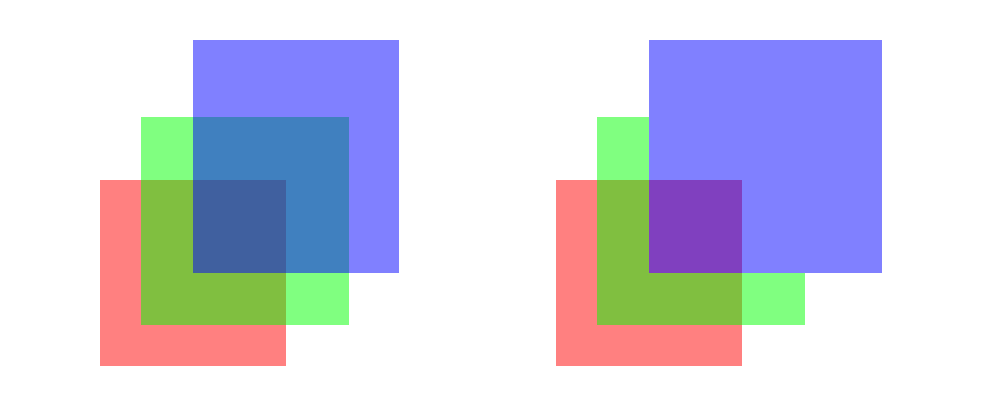
\includegraphics[width=\columnwidth]{oit_example.png} 
	 \caption[Order Independent Transparency]{The left image is rendered in
	 correct back-to-front order. The right image is out-of-order, the green
	 square does not properly blend into the blue square.}
	 \label{figure:oit}
	\end{figure}
    % =============


\subsection{Effects}
Here we briefly discuss our usage of graphical effects. OIT rendering, as
described above, is used to ensure correct depth cues, it is possible to achieve
different look and feel by passing different lighting equations to the shader
programs. Halo effect is done by calculating silhouettes in \twod space of the
active entities, we then subtract the geometric shape from the silhouette, and
perform a smoothing step to blur out sharp features on the outline. The ghostly
outline effect is done by calculating ridge and silhouette edges of adjacency
structures in the mesh, as outlined in Hermosilla's GPU implementation
\cite{Hermosilla2009}. Finally the lens effect is achieved through adding and
subtracting of textures, the full scenes with lens semantic is rendering into a
texture, we alter the non-lens area to be completely transparent and superimpose
the remainder onto the existing scene.



\subsection{Cache and Stabilization}
Due to the size of our data and the diverse variations of queries on the database, 
we have encountered situations where our database does not produce a stable 
performance. We have found with SQL queries alone our query results come back 
between several milliseconds to a few seconds. A major part of this delay is due 
to the nature of the queries, which are mostly aggregates that result in sorting 
operations. We found this to be unacceptable, because it defies people�s 
expectation of instantaneous reaction from the system.

To create a better user experience in-line with user expectations, we created
a hierarchical lookup table that partially caches the aggregated query results. 
Each level corresponds to a unique filtering criteria based on our dataset, for 
this prototype, we have from highest level to lowest level : time, entity, 
manufacturer, make, model and year. The hierarchy order models the type of 
successive query refinement we expect of typical interactions. Each entry, in any 
level, corresponds to the aggregated query up to that specific point. Each entry 
contains a value that is the aggregated count of the documents, as well as a 
reference to a list of its children, if applicable. For example: (``2000'',
``engine'', ``Toyota'') will yield the query results of all Toyota vehicle
complaints that had engine problems in the year 2000. To create ranged query, for example 2000 to 2005, we 
issue the same query with different time parameters and sum up the results. More 
complex queries such as aggregation and co-occurrences, are done in similar manner, 
but with different lookup tables. In practice, we found this to be a middle of the 
road approach. Comparing to raw database queries, it performs slower than best case 
but much faster than the worst case scenarios, most important of all, we have 
consistent performance at around 100 to 200 millisecond, which we found to be 
acceptable for interactive use.

The table is created at when system starts, we iterate through the database
tables once, creating the hierarchy structure and increment the counts as we go. As a last 
optimization step, we have attempted to serialize out the query tables to disk, 
so they can be de-serialized on system startup without having to iterate the
database tables. However, without a customized data container, this in practice turned out 
to be slower than database lookups and was abandoned.


\subsection{Multi-Touch Heuristics}
Touch sensors have a few drawbacks, there are inherent noises that come from
performing gestures, in addition, our inability to hold our hands perfectly
still accentuate this issue by create jitters. In our particular use case, the
upright display makes certain gestures difficult, for example, in our informal
evaluation of the display we found that certain curvatures of sinusoidal curves
introduced noises because the knuckles of other fingers are sensed as
unintended touch points as a result of drifting too lose to the screen itself.

These noises degrades user experiences, as they trigger unexpected events within
the system. We introduce a set of software heuristics as an intermediate step
between when the points are sensed and when they are executed. In general, these
heuristics remove unintended touches and prevent jittery graphics as a result of
minute movements. While these are tuned specifically for our hardware, we
believe rules are general enough that they can be adopted to other touch
sensors. 

\begin{itemize} [noitemsep]
  \item \textbf{Real Update:} The muscle deformation when pressed against the
  display, paired with inability to keep perfect still postures results in
  sensor registering jittery updates. This is undesirable because it induces a
  shaking effect, and often time unnecessary because the updates are minute.
  To compensate this problem, we only accept an update if it is at least 2
  number of pixels away from the previous update point.
  
  \item \textbf{Coincidental Points:} When a touch is initialized on the touch
  surface, there is a possibility that more than one touch point will be
  registered. This is similar to the case we presented above. To reduce this scenario from
  occurring, we store the xy-coordinate and the time the touch point is created.
  If a touch point is created too close to any other touch point within a time
  threshold, that point is rejected
  
  \item \textbf{Movement Buffer:} When a gesture is in transition, there are
  cases where other parts of the hand will inadvertently cause new points. We
  try to neutralize these occurrences by introducing buffer zones around touch
  points in transition. New touch points cannot be created in the zones, however
  existing touch points are not affected.
  
  \item \textbf{Reinforce Intention:} This heuristic deals with reducing jitters
  on the initial touch. This can be seen as a special case of the Real Update
  heuristic, but while Real Update toss away extremely small update in general,
  the first update can be quite large, probably due to the act of pressing the
  finger against the display. We made is such that the first update must be at
  least 20 pixels distance in magnitude. This heuristic is not applicable to
  lens widget nor document widget because we want them to be immediately
  responsive.
  
\end{itemize}


